\documentclass[sigconf,authorversion]{acmart}
\usepackage[utf8]{inputenc}
\usepackage{booktabs}
\usepackage{enumitem} %resume enumerate
\usepackage{graphicx}
\usepackage{caption}
\usepackage{subcaption}

% Remove reference format
\settopmatter{printacmref=false}
\setcopyright{none}
\renewcommand\footnotetextcopyrightpermission[1]{}
\pagestyle{plain}

\title{Clustering Algorithms for Color Segmentation}
\author{Roger Pujol}
\affiliation{%
  \institution{Universitat Politècnica de Catalunya (UPC)}
  \city{Barcelona}
  \country{Spain}}
% \affiliation{%
%   \institution{Barcelona Supercomputing Center (BSC)}
%   \city{Barcelona}
%   \country{Spain}}
\email{roger.pujol.torramorell@est.fib.upc.edu}
\date{\today}

\begin{abstract}
Clustering Algorithms are an interesting powerful tool, that in many cases doesn't need a lot of parameters in order to get useful results. Another intriguing thing about these algorithms is that most of them are unsupervised, which means that the results can easily be unexpected. In this project we will apply them to the colors of some images, to see how different algorithms and different color-spaces affect to the way to find the most important colors of an image.\\
The code of this project is Open Source and can be found in: \url{https://github.com/rogerpt32/adm_paper2}
\end{abstract}

\begin{document}

\maketitle

\section{Introduction}
In this project we are going to apply three different clustering methods (k-means, EM(GMM) and BIRCH) in two particular color-spaces (RGB and HSV) for various images. With this we want to see the impact to the results of each algorithm and compare them. Also will be interesting to see how different representations of the same data can affect to the results.\\
\emph{Note: In this report, I only show a very small portion of the results because of some space limitation and to simplify the comprehension. I strongly recommend to download the source code and then check all the outputs and even run the ``getall.sh'' script to get the complete outputs.}

\section{Data Description}
The data we used to test test the algorithms are 4 pictures that are usually used as Test Images (see Figure \ref{fig:original}).
\begin{figure}[hbtp]
  \begin{subfigure}[b]{0.45\columnwidth}
      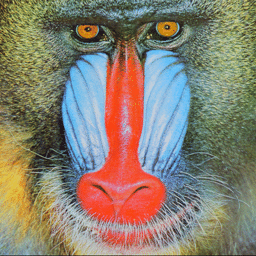
\includegraphics[width=\columnwidth]{../imgs/baboon.png}
      \caption{``baboon.png''}
      \label{subfig:baboon}
  \end{subfigure}
  \hspace{0.01\textwidth}
  \begin{subfigure}[b]{0.45\columnwidth}
      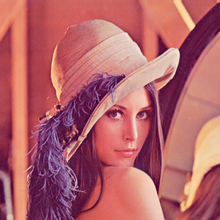
\includegraphics[width=\columnwidth]{../imgs/lena.png}
      \caption{``lena.png''}
      \label{subfig:lena}
  \end{subfigure}
  \hspace{0.01\textwidth}
  \begin{subfigure}[b]{0.45\columnwidth}
    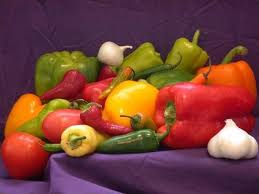
\includegraphics[width=\columnwidth]{../imgs/peppers2.jpeg}
    \caption{``peppers2.jpeg''}
    \label{subfig:peppers2}
  \end{subfigure}
  \hspace{0.01\textwidth}
  \begin{subfigure}[b]{0.45\columnwidth}
      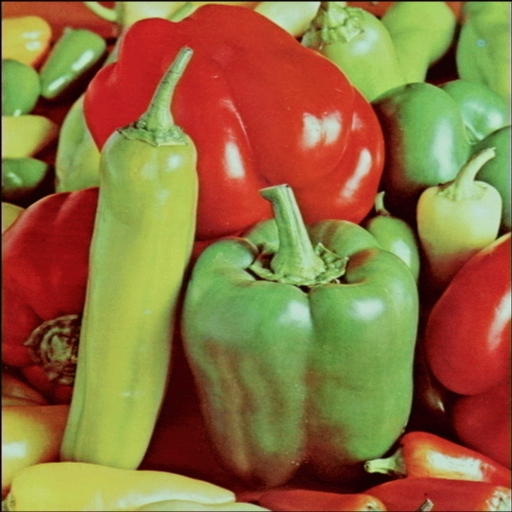
\includegraphics[width=\columnwidth]{../imgs/peppersc.jpg}
      \caption{``peppersc.jpg''}
      \label{subfig:peppersc}
  \end{subfigure}
  \caption{Images used as Data in this project}
  \label{fig:original}
\end{figure}
For each of these pictures we generated a Dataset where each row represents a pixel with the following variables:
\begin{itemize}
  \item \textbf{X}: The position of the pixel in the image in the X axis.
  \item \textbf{Y}: The position of the pixel in the image in the Y axis.
  \item \textbf{R}: The component R of the pixel in the RGB color-space.
  \item \textbf{G}: The component G of the pixel in the RGB color-space.
  \item \textbf{B}: The component B of the pixel in the RGB color-space.
  \item \textbf{H}: The component H of the pixel in the HSV color-space.
  \item \textbf{S}: The component S of the pixel in the HSV color-space.
  \item \textbf{V}: The component V of the pixel in the HSV color-space.
\end{itemize}

\subsection{RGB color-space}
The RGB color-space is a structure to define any color describing it in 3 basic colors: Red, Green and Blue. Each of the components usually have values between 0 and 255 or between 0 and 1.

\subsection{HSV color-space}
The HSV color-space is a structure to define any color describing it in 3 basic features: Hue, Saturation and Value. The Hue is an angle usually represented in degrees (0 to 360) or in radiants (0 to $2\pi$) that represents the base color. The Saturation is a value that represents the intensity of the color where 0 would be whites, grays and blacks, and 1 mean maximum intense color like could be a pure green (in RGB 0,255,0). Finally the Value is the brightness of the color where 0 is absolute black and 1 would be absolute white (if $S=0$) or a bright color like the green mentioned before.

\section{Preprocess}
The only preprocess of the data that has to be done is a transformation at the HSV color space. In this project we will ignore the V value in order to try segmenting ignoring if the color in the image is properly illuminated. As stated before, the H and the S are an angle and a radius, like polar coordinates. This is not a good way to represent something if you want to cluster it, so what we did is parse it to a 2D plane with kind of cartesian coordinates.

\section{Algorithms}
This section describes briefly the algorithms used.
\subsection{K-Means}
The K-Means algorithm seeks to cluster the data in a given number of groups ($k$ groups). In order to do it, the algorithm starts selecting randomly $k$ centers, then it assigns each point to the nearest center and calculates the mean for every group. Then this step is repeated with the means as new centers. This process is done until the centers stabilize. The final output are the centers and each point is assigned to the nearest one.
\subsection{EM (Gaussian Mixture Model)}
EM (Expectation Maximization) with Gaussian Mixture Model, tries to find $k$ groups by assigning to each of them a Gaussian Distribution. The final groups are accepted when the expectation of all the distributions reach a maximum.
\subsection{BIRCH}
BIRCH algorithm, first builds a CF Tree with the data. Then it applies K-Means or another clustering to the Tree to get the final clusters.

\section{Postprocess}
In order to see how the results affects to the original image, we have to postprocess the output.\\
For the RGB framework is simple, we only have to get the mean (center) color of the cluster and create a new image where each pixel has the value of the center of the cluster that has assigned to it.\\
For the HSV we have to do the same but firs we should pass the centers from cartesian coordinates to the regular HS(V) color-space and then use that to convert it to RGB. Since we deleted the value (V) of the color-space to ignore light differences, the result also lacks of this feature, then in order to get a RGB color we will have to fix a brightness value. The value chosen is almost full brightness, since this will be usefull to show more clearly the colors.

\section{Results}
Now I will provide some of the tests that had major differences in the results with each algorithm and color-spaces.
\subsection{Comparing Algorithms}
Clustering the colors of the image Baboon with only 2 clusters with the three algorithms will output three very different outputs (see Figures \ref{fig:baboon_2_hsv} and \ref{fig:baboon_2_rgb}). In these figures we can appreciate how EM successfully divide 2 clear groups which are an intense Red and a Green. K-Means and BIRCH have very similar results in the HSV color-space but different in RGB, here the group of points detected by EM falls almost entirely to different clusters. In this particular case, EM seems to get the two most human intuitive clusters and the other methods are only dividing the data almost through the middle.

\subsection{Comparing Color-Spaces}
To compare the color-spaces we will focus on Figure \ref{fig:peppers_5}. Ignoring the fact that the colors in the of HSV are a lot brighter, because we added that bright afterwards, the color clusters are very different. Since we deleted the bright feature in the HSV, it seems that the colors almost fits perfectly for each object ignoring completely the shadows and other light effects, on the other hand RGB captures all the shadows as different colors and this mixes the objects from the original picture. Probably with this we could say that using our HS(V) color-space, we could segmentate objects based on their color.
\begin{figure}[hbtp]
  \begin{subfigure}[b]{0.45\columnwidth}
      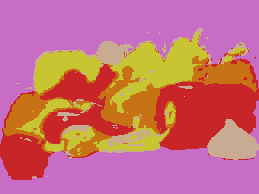
\includegraphics[width=\columnwidth]{../outputs/peppers2_5_hsv_colored_kmeans.png}
      \caption{Colored HSV image with K-Means}
      \label{subfig:peppers_hsv_kmeans}
  \end{subfigure}
  \hspace{0.05\columnwidth}
  \begin{subfigure}[b]{0.45\columnwidth}
      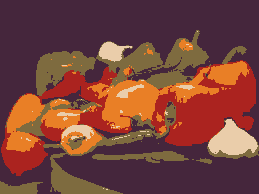
\includegraphics[width=\columnwidth]{../outputs/peppers2_5_rgb_colored_kmeans.png}
      \caption{Colored RGB image with K-Means}
      \label{subfig:peppers_rgb_kmeans}
  \end{subfigure}

  \begin{subfigure}[b]{0.45\columnwidth}
      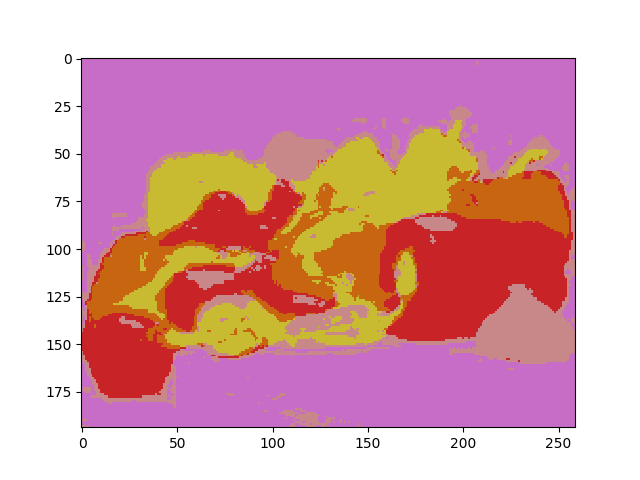
\includegraphics[width=\columnwidth]{../outputs/peppers2_5_hsv_colored_gmm.png}
      \caption{Colored HSV image with EM}
      \label{subfig:peppers_hsv_gmm}
  \end{subfigure}
  \hspace{0.05\columnwidth}
  \begin{subfigure}[b]{0.45\columnwidth}
      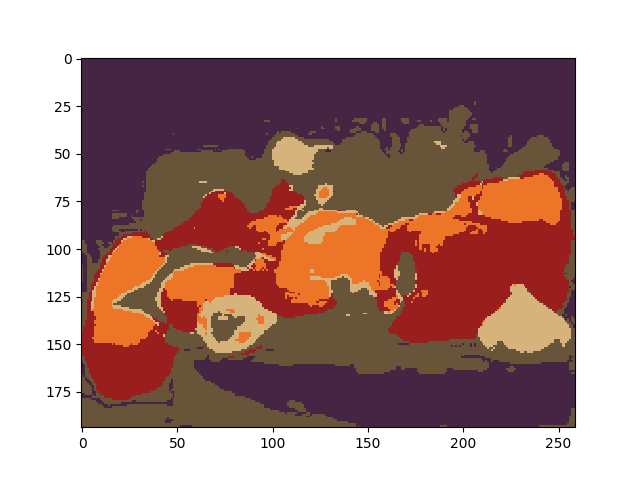
\includegraphics[width=\columnwidth]{../outputs/peppers2_5_rgb_colored_gmm.png}
      \caption{Colored RGB image with EM}
      \label{subfig:peppers_rgb_gmm}
  \end{subfigure}

  \begin{subfigure}[b]{0.45\columnwidth}
      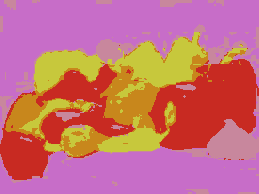
\includegraphics[width=\columnwidth]{../outputs/peppers2_5_hsv_colored_birch.png}
      \caption{Colored HSV image with BIRCH}
      \label{subfig:peppers_hsv_birch}
  \end{subfigure}
  \hspace{0.05\columnwidth}
  \begin{subfigure}[b]{0.45\columnwidth}
      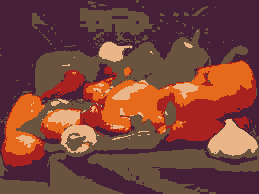
\includegraphics[width=\columnwidth]{../outputs/peppers2_5_rgb_colored_birch.png}
      \caption{Colored RGB image with BIRCH}
      \label{subfig:peppers_rgb_birch}
  \end{subfigure}
  \caption{Peppers2 image colored  using every algorithm with 5 clusters in a RGB and HSV color-space}
  \label{fig:peppers_5}
\end{figure}

\section{Conclusions}
At the end of the experiments, it looks like all the algorithms achieve to get coherent groups in most of the situations and the correctness of one method over another depend mostly in the data used. Also we have found that if we want to segmentate objects in an image knowing their color, HSV will probably be a better color-space to do it, since we can toggle off the brightness of the image and focus only on the color.

\begin{figure*}[hbtp]
  \begin{subfigure}[b]{0.25\textwidth}
      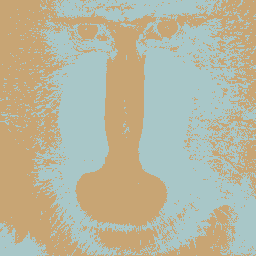
\includegraphics[width=\textwidth]{../outputs/baboon_2_hsv_colored_kmeans.png}
      \caption{Colored image with K-Means}
      \label{subfig:baboon_hsv_kmeans}
  \end{subfigure}
  \hspace{0.05\textwidth}
  \begin{subfigure}[b]{0.25\textwidth}
      
\includegraphics[width=\textwidth]{../outputs/baboon_2_hsv_colored_gmm.png}
      \caption{Colored image with EM}
      \label{subfig:baboon_hsv_gmm}
  \end{subfigure}
  \hspace{0.05\textwidth}
  \begin{subfigure}[b]{0.25\textwidth}
      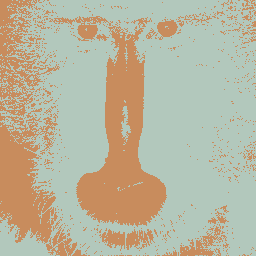
\includegraphics[width=\textwidth]{../outputs/baboon_2_hsv_colored_birch.png}
      \caption{Colored image with BIRCH}
      \label{subfig:baboon_hsv_birch}
  \end{subfigure}
  \begin{subfigure}[b]{0.25\textwidth}
      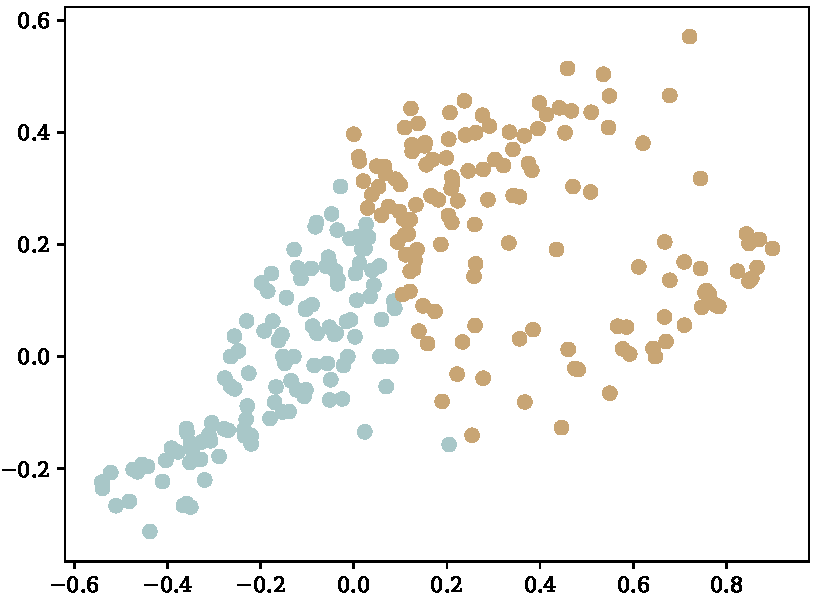
\includegraphics[width=\textwidth]{../outputs/baboon_2_hsv_plot_kmeans.pdf}
      \caption{Color-space plot with K-Means}
      \label{subfig:p_baboon_hsv_kmeans}
  \end{subfigure}
  \hspace{0.05\textwidth}
  \begin{subfigure}[b]{0.25\textwidth}
      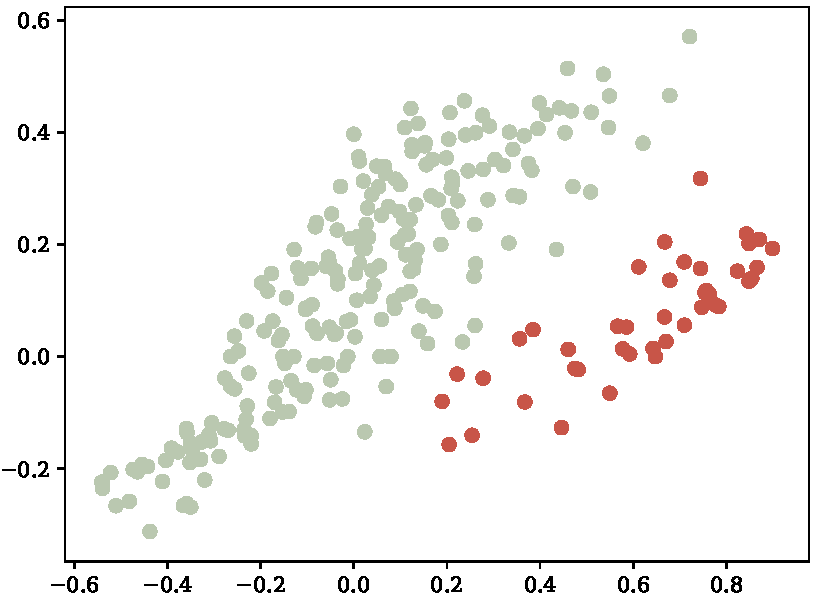
\includegraphics[width=\textwidth]{../outputs/baboon_2_hsv_plot_gmm.pdf}
      \caption{Color-space plot with EM}
      \label{subfig:p_baboon_hsv_gmm}
  \end{subfigure}
  \hspace{0.05\textwidth}
  \begin{subfigure}[b]{0.25\textwidth}
      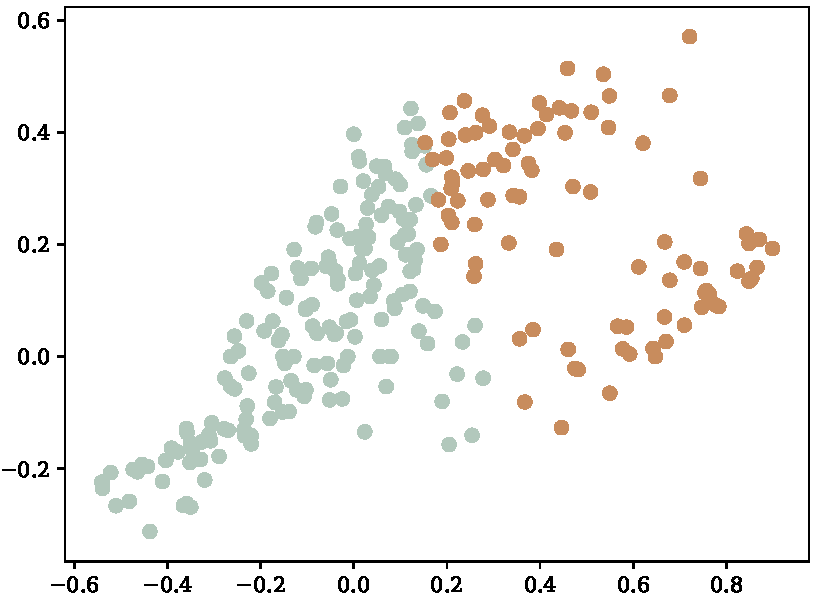
\includegraphics[width=\textwidth]{../outputs/baboon_2_hsv_plot_birch.pdf}
      \caption{Color-space plot with BIRCH}
      \label{subfig:p_baboon_hsv_birch}
  \end{subfigure}
  \caption{Baboon image colored and its plot using every algorithm with 2 clusters in a HS(V) color-space}
  \label{fig:baboon_2_hsv}
\end{figure*}

\begin{figure*}[hbtp]
  \begin{subfigure}[b]{0.25\textwidth}
      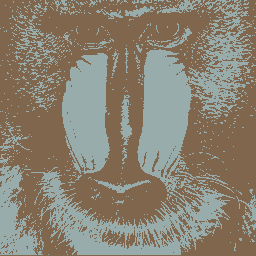
\includegraphics[width=\textwidth]{../outputs/baboon_2_rgb_colored_kmeans.png}
      \caption{Colored image with K-Means}
      \label{subfig:baboon_rgb_kmeans}
  \end{subfigure}
  \hspace{0.05\textwidth}
  \begin{subfigure}[b]{0.25\textwidth}
      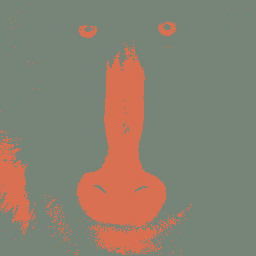
\includegraphics[width=\textwidth]{../outputs/baboon_2_rgb_colored_gmm.png}
      \caption{Colored image with EM}
      \label{subfig:baboon_rgb_gmm}
  \end{subfigure}
  \hspace{0.05\textwidth}
  \begin{subfigure}[b]{0.25\textwidth}
      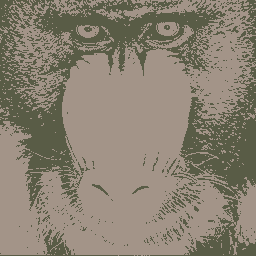
\includegraphics[width=\textwidth]{../outputs/baboon_2_rgb_colored_birch.png}
      \caption{Colored image with BIRCH}
      \label{subfig:baboon_rgb_birch}
  \end{subfigure}
  \begin{subfigure}[b]{0.25\textwidth}
      \includegraphics[width=\textwidth]{../outputs/baboon_2_rgb_plot_kmeans.pdf}
      \caption{Color-space plot with K-Means}
      \label{subfig:p_baboon_rgb_kmeans}
  \end{subfigure}
  \hspace{0.05\textwidth}
  \begin{subfigure}[b]{0.25\textwidth}
      \includegraphics[width=\textwidth]{../outputs/baboon_2_rgb_plot_gmm.pdf}
      \caption{Color-space plot with EM}
      \label{subfig:p_baboon_rgb_gmm}
  \end{subfigure}
  \hspace{0.05\textwidth}
  \begin{subfigure}[b]{0.25\textwidth}
      \includegraphics[width=\textwidth]{../outputs/baboon_2_rgb_plot_birch.pdf}
      \caption{Color-space plot with BIRCH}
      \label{subfig:p_baboon_rgb_birch}
  \end{subfigure}
  \caption{Baboon image colored and its plot using every algorithm with 2 clusters in a RGB color-space}
  \label{fig:baboon_2_rgb}
\end{figure*}

% \bibliographystyle{unsrt}
% \bibliography{cites}

\end{document}
